\documentclass{article}

% if you need to pass options to natbib, use, e.g.:
% \PassOptionsToPackage{numbers, compress}{natbib}
% before loading nips_2017
%
% to avoid loading the natbib package, add option nonatbib:
% \usepackage[nonatbib]{nips_2017}

\usepackage{nips_2017}

% to compile a camera-ready version, add the [final] option, e.g.:
% \usepackage[final]{nips_2017}

\usepackage[utf8]{inputenc} % allow utf-8 input
\usepackage[T1]{fontenc}    % use 8-bit T1 fonts
\usepackage{hyperref}       % hyperlinks
\usepackage{url}            % simple URL typesetting
\usepackage{booktabs}       % professional-quality tables
\usepackage{amsfonts}       % blackboard math symbols
\usepackage{nicefrac}       % compact symbols for 1/2, etc.
\usepackage{microtype}      % microtypography
\usepackage{graphicx}
\usepackage{amsmath, amssymb, amsthm, epsfig}

\usepackage{enumitem}
\setlist[itemize]{leftmargin=-5ex}
\setlist[itemize]{itemsep=-1ex}

\title{Toward Goal-Driven Neural Network Models for Rodent Whisker-Trigeminal System}

\author{
Chengxu Zhuang\\
Department of Psychology\\
Stanford University\\
Stanford, CA 94305 \\
\texttt{chengxuz@stanford.edu} \\
\And
Jonas Kubilius \\
Department of Brain and Cognitive Sciences \\
Massachusetts Institute of Technology \\
Cambridge, MA  02139\\
\texttt{qbilius@mit.edu} \\
\And
Mitra Hartmann \\
Departments of Biomedical Engineering \\
and Mechanical Engineering \\
Northwestern University \\
Evanston, IL  60208\\
\texttt{hartmann@northwestern.edu} \\
\And
Daniel Yamins \\
Departments of Psychology and Computer Science \\
Stanford Neurosciences Institute \\
Stanford University \\
Stanford, CA 94305 \\
\texttt{yamins@stanford.edu} \\
}


\begin{document}
% \nipsfinalcopy is no longer used

\maketitle

\begin{abstract}
Abstract
\end{abstract}

%Papers may be only up to eight pages long, including figures.
%An additional ninth page containing only cited references is allowed.

\section{Introduction} %~750 words
%sensory systems generally
The sensory systems of brains do remarkable work in extracting behaviorally useful information from noisy and complex raw sense data. 
Vision systems process retinal photoreceptor intensity arrays, auditory systems interpret hair-cell displacement amplitudes, and somatosensory systems integrate data from direct physical interactions.~\cite{purves2001neuroscience} 
While these systems differ radically in their input modalities, number of overall neurons, specific neuronal microcircuits, and across species, they share two fundamental characteristics. 
First, they are hierarchical sensory cascades, consisting of sequences of brain areas (cortical and subcortical), that together produce a complex transformation of the input data.  
Second, they operate in inherently highly-structured spatiotemporal domains, and are often known to be laid out in the brain in maps reflecting this structure~\cite{felleman1991distributed}.

Extensive experimental work in rodent barrel/somatosensory cortex has provided insights into how these principles help the rodent use their whiskers to learn about the objects in their environment.  
Similar to the ventral stream of visual systems with hierarchical structures from V1, to V2, V4, and IT~\cite{felleman1991distributed, Goodale1992}, researchers have found evidence of hierarchical processing for somatosensory input in rodents, human, and primates\cite{Pons1987, Inui2004, Iwamura1998}. 
For example, the second somatosensory area (S2) is found to rely on inputs from S1 (first somatosensory area) \cite{Pons1987, Petersen2007}. 
Barrel cortex, S1, and S2 accept input from subcortical cascade driven by  whiskers input \cite{Diamond2008}. 
However, while the rodent somatosensory system has been the subject of extensive experimental efforts\cite{armstrong1992flow, petersen2003spatiotemporal, kerr2007spatial, von2007neuronal}, there have been comparatively few attempts at computational modeling of this important sensory area. 

Recent work has shown that deep neural networks (DNNs), which have hierarchy and spatial structure built into their architectures, can be effective models of neural processing in vision\cite{cadieu2014deep, Yamins2014} and audition\cite{kell_yamins_sfn}.
Motivated by these successes and by the known structure of rodent barrel cortex, in this work we illustrate initial steps toward using DNNs to model rodent somatosensory systems.
Our driving hypothesis is that rodent barrel cortex is optimized to use whisker-based sensor data to solve somatosensory tasks in complex, variable real-world environments. 
The basic idea in our approach is thus to use \emph{goal-driven} modeling (Fig \ref{fig_schematic}), in which the DNN parameters --- both discrete and continuous --- are optimized for performance on a challenging ethologically-relevant task\cite{yamins2016using}.  
Insofar as the shape recognition task is a strong constraint on network parameters, the resulting optimized neural network may be an effective model of real barrel cortex neural response patterns. 
 
\begin{figure}
\centering
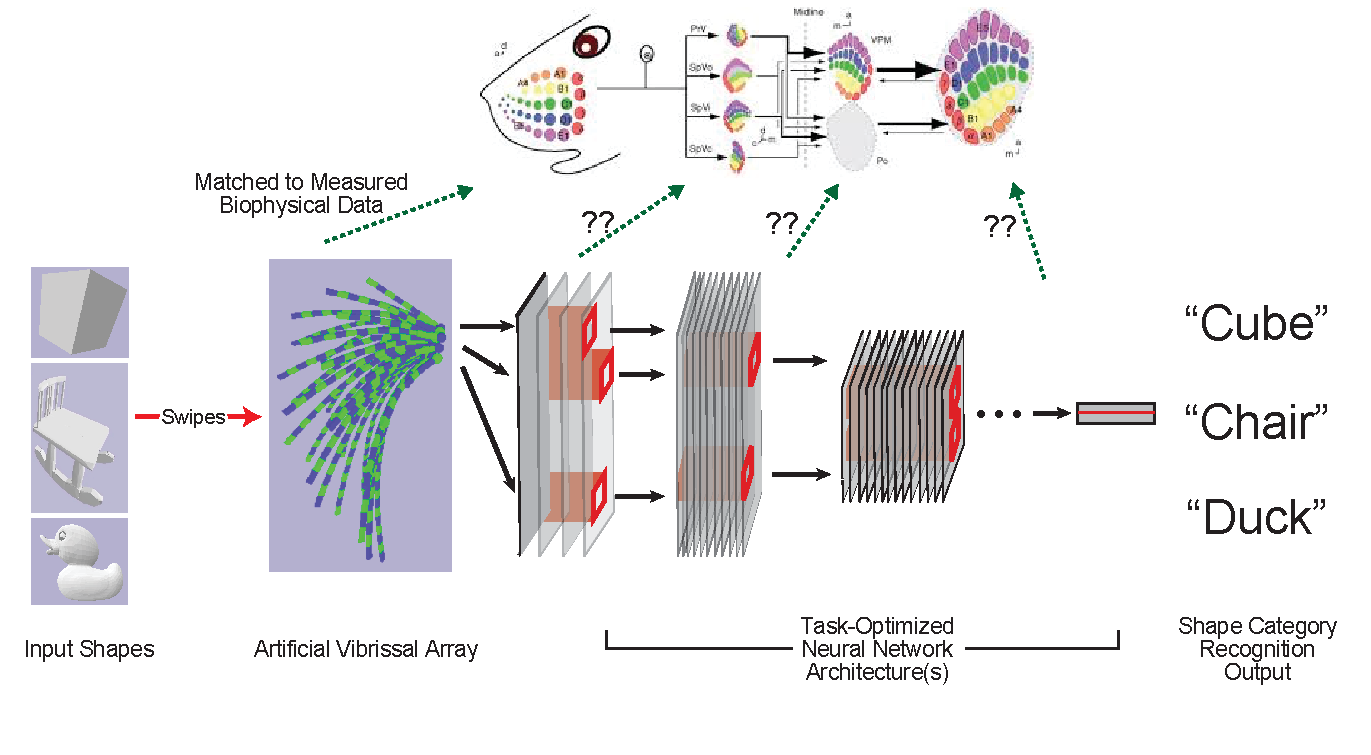
\includegraphics [width=1\linewidth]{figures/schematic.pdf}
\vspace{-2mm}
\caption{\textbf{Goal-Driven Approach to Modeling Barrel Cortex:} \textbf{a.} Rodents have highly sensitive whisker arrays that provide input data about the animal's environment.  Whisker signals are is subsequently processed by a somatosensory cascade of brain areas knowns as barrel cortex. Barrel cortex is a prime target for modeling because it is likely to be richly representational, but its computational underpinnings are largely unknown. Our long-term approach to modeling barrel cortex is \emph{goal-driven}: using an artificial whisker-array input device built using extensive biophysical measurements (\textbf{b.}), we seek to optimize neural networks of various architectures (\textbf{c.}) to solve ethologically-relevant shape recognition tasks (\textbf{d.}), and then measure to what extent the networks predict fine-grained response patterns in real neural recordings. ~\label{fig_schematic}}
\end{figure}

This idea is conceptually straightforward, but implementing it involves surmounting several major challenges.  
Unlike the cases of vision or audition, where the contents of the retina or cochlea can for many purposes be approximated by a mathematically simple data array (namely, a uniform data array representing light or sound intensities), the equivalent mapping between stimuli (e.g. objects in a scene) and the sensor input to the whisker system is much less direct.   
Thus, a biophysically-realistic embodied model of the whisker array is a critical first component of any barrel cortex model.
Once the sensor is available, a second key problem is building a neural network that can accept whisker data input and use it solve relevant tasks. 
Aside from the question of the neural network design itself, knowing what the ``relevant tasks'' are for training a rodent whisker system, in a way that is sufficiently concrete to be practically actionable, is a significant unknown, given the very limited amount of ethologically-relevant behavioral data on rodent sensory capacities\cite{von2007neuronal, Knutsen2006, OConnor2010, Arabzadeh2005, Diamond2008}.
Collecting neural data of sufficient coverage and resolution to quantitatively evaluate one or more task-optimized neural network models represents a third major challenge.   

In this work, we show initial steps on the first two of these problems (sensor modeling and neural network design/training). 





\section{Modeling the Whisker Array Sensor} %~500 words
\begin{figure}
\centering
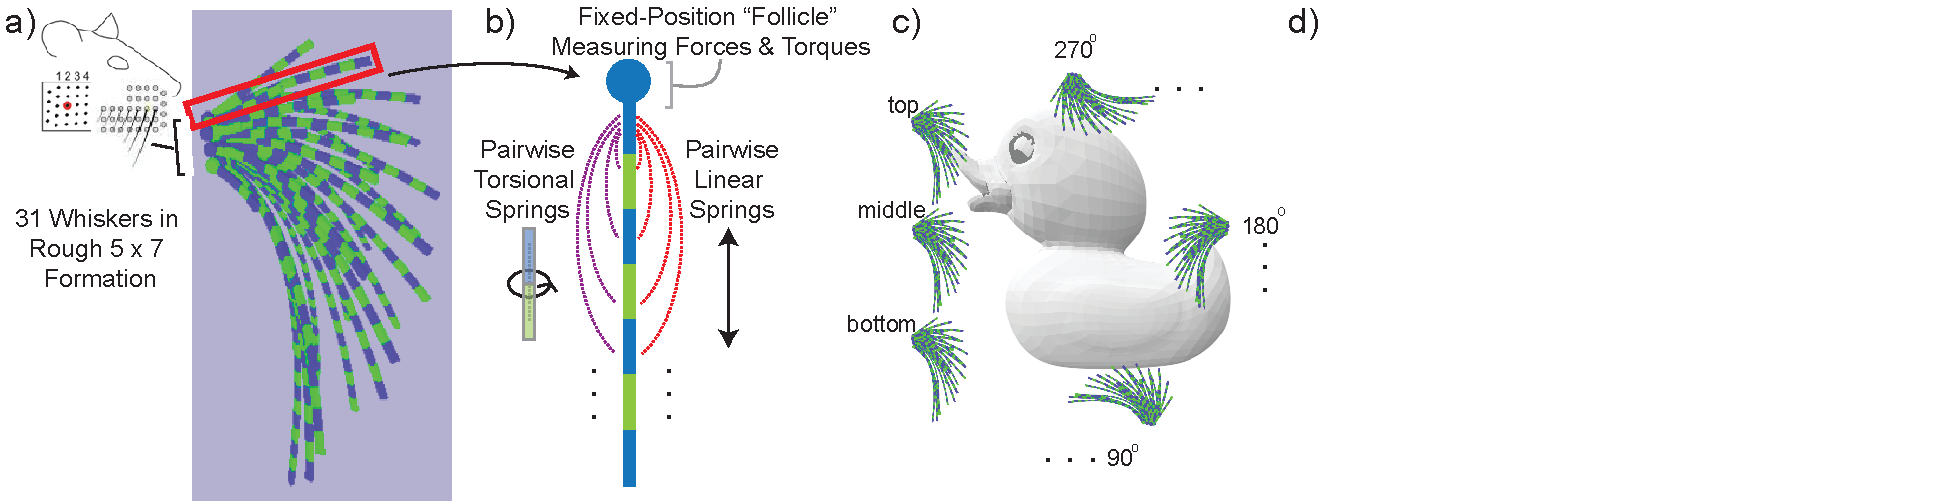
\includegraphics [width=1\linewidth]{figures/whiskers.pdf}
\vspace{-2mm}
\caption{\textbf{Dynamic Three-Dimensional Whisker Model:} \textbf{a.} We constructed an array of 31 whisker objects, arranged in a 5x7 grid (with 4 missing elements).  Whisker number, placement, length and static shape were matched to biophysical data. \textbf{b.} Each whisker element is composed of a set of cuboid objects.  The follicle cuboid has a fixed location, and is attached to movable cuboids making up the rest of the hair. Motion is constrained by linear and torsional springs between each pair of cuboid elements.  The parameters of these springs are chosen to ensure naturalistic motion of the whiskers.  \textbf{c.} During dataset construction, the whisker is brought into contact with each object at three vertical heights (top, middle bottom), at each of 4 90-degree separated attack angles, for a total of 12 swipes.  Object initial angle, size, and swipe speed vary randomly between each group of 12 swipes.  Forces and torques are recorded at the three cuboids closest to to the follicle, for a total of 18 measurements per whisker per timepoint.  \textbf{d.} ~\label{fig_whiskers}}
\end{figure}

In order to provide the similar inputs to deep neural networks as those to rodent somatosensory systems, one will need a physically accurate models for the the rodent whiskers.
In our models, we are more interested in ensuring the correctness of the mechanical details of every individual whisker.
And at the same time, we also need the simulations to be fast enough for generating a large scale dataset.
Therefore, we use Bullet~\cite{wiki:bullet} as physics engine, which is a open-source real-time physics engine used in many video games and visual effects in movies.
Meanwhile, we also need to make our model biologically accurate. So the parameters used in our model including position, curvature, and length of each whisker, are from biological static whisker model in~\cite{Towal2011}.

We use small cuboids concatenated along the longest dimension to model single whisker, where each cuboid is connected to every other cuboid in the same whisker using both linear and torsion springs.
The equilibrium points of all the springs as well as the initial positions of all cuboids are set to make the whiskers fit the required curvature.
Each cuboid is in the same shape with the length of 2mm and the number of cuboids is chosen to fit the required length for different whisker.
The bottom of whiskers will be fixed at the given positions. Except that, the motion of every cuboid is only constrained by the springs connecting to it.
Besides, there is no collision between cuboids in different whiskers or in the same whisker.
And in our simulation, we only used right whisker array.

As we are simulating the whiskers using concatenated cuboids and the dynamics of the physics engine is calculated frame by frame and kept the same between frames, we can not derive stiffness of springs between cuboids directly from dynamic related parameters of whiskers.
In addition, we need to add damping to cuboids, which means that their motion will be decayed at a fixed rate every frame. Otherwise the cuboids can not stop their motions.
As it's hard to derive those parameters from biological models, we use optimization method to find the best values maximizing the "reasonability" of the dynamic behaviors of whiskers.
Specifically, for each whisker, we construct four situations where four forces are applied to the end of that whisker for a fixed amount of time.
These four situations include pushing whisker towards the bottom, pushing whisker forward, pushing whisker forward further, and pushing whisker to its left.

For each simulatin, we simulate the process that the whisker recover to the static position after applying the force and then measure the time ($T$) needed for recovery, the distance ($S$) travelled by all cuboids between the end of applying the force and recovery, the distance ($d$) between the bottom and the end of the whisker at the end of applying the force, and the average speed ($v$) of all cuboids during the recovery.
We use hyperopt~\cite{bergstra2013hyperopt} for optimizing those hyper parameters including damping and spring stiffness. The optimization is done to every whisker independently as the hyper parameters are not shared between whiskers.
In order to reduce the number of parameters we need to optimize, we assume that within one whisker, all cuboids shares the same damping setting including linear damping and rotation damping.
Furthermore, we group the springs by the their length, which means that the spring connecting 1st cuboid and 3rd cuboid as well as the spring connecting 2st cuboid and 4th cuboid and so on will be in the same group.
For each group, we assume that the stiffness is linearly correlated with the distance between the starting cuboid of this spring and the bottom of that whisker.
This is inspired by the fact that the whisker will be thicker and stiffer at the bottom~\cite{Hartmann:2015}.
And finally, we set our loss function to be $0.025S + d + 20T - 2v$, where the coefficients are set to make each term comparable.
The hyperopt program will try to find the best hyper parameters to minimize the loss function, which means that after applying a fixed amount of force, we expect the whisker to recover as fast as we can (positive coefficients for $S$, $T$, and $v$) and also the stiffness not being so large that the whisker can not be bent (negative coefficient for $d$).

Finally, we have a whisker array consisting of 31 whiskers whose bottoms are placed on a surface of ellipsoid in a grid of $5\times7$ with some vacant positions, where the longest whisker has around 30 cuboids and shortest whisker has around 4 cuboids. 


\section{A Large-Scale Whisk Dataset} %~750 words
After we have the whisker array, we can generate a large-scale dataset for training the neural networks by simulating the mice using whiskers for some specific tasks.
The choice of the tasks is believed to be critical for whether the trained networks will be a good model for that cortex or not.
For example, it has been shown that one of the imporant reasons that the neural networks trained for object recognition could predict responses of IT cortex in visual cortex well~\cite{cadieu2014deep, Yamins2014} is that object recognition is believed to be a major function performed by IT cortex~\cite{hung2005fast, yamins2016using}.
Although the functions performed by rodent somatosensory systems are poorly understood, it is found that rodents could use their whiskers to detect object shape, position, and texture of object surface\cite{Boubenec2012,Diamond2008,Arabzadeh2005,OConnor2010}
Therefore, we are temporarally using object recognition as the task to generate the dataset and optimize the neural networks. 
Meanwhile, we also make other information such as object shapes as surface normals and speed of object moving available for further task switching.

Specifically, the dataset we generated consists of many independent trails in which one object will be moving towards the whisker array from the front of it in a constant speed.
The collision happens between object and cuboids while the speed of object will not be influenced.
For every whisker, we collect the sums of all the forces and torques from all springs connecting to three cuboids respectively at the bottom of that whisker, as researchers have found that forces and torques can be used to explain the signals transimitted by follicles of whiskers~\cite{Quist2014, Huet2016}.

The objects used are chosen from ShapeNet~\cite{Chang2015}, where over 50 thousand 3D objects belonging to 55 categories are collected from Internet. 
We further split the 55 categories into 117 categories by extracting fine-grained subcategories. 
Then we randomly sample 9981 objects from ShapeNet with much more averaged category distribution, where most of the categories as well as the categories with most objects have 91 objects and the category with fewest objects has 42 objects. 



\section{Computational Architectures} %~1250 words
In this section, we will show several families of DNNs trained on the dataset. Different families of DNNs are based on different hypotheses about the computations performed by neurons. 
For example, the model with spatial-temporal convolution structure is based on our assumption about neurons integrating spatial-temporal information. 
As the temporal dimension of our input data is fixed across different trials, we could use feed-forward convolutional neural networks (CNNs) as well as recurrent neural networks (RNNs).
We will compare different families of networks through their performances while controlling the number of parameters in the model.

\subsection{Spatial-temporal integrating networks}

In this family of networks, we use CNNs where convolution is done both on temporal dimension and spatial dimension, which means that responses from different whiskers across some time will be combined together in neurons of every layer, while neurons at higher layer will have larger receptive field on both dimensions.


\subsection{Temporal integrating before spatial integrating}

\subsection{Spatial integrating before temporal integrating}

\subsection{Recurrent neural networks}

\section{Results} %~500 words
\begin{figure}
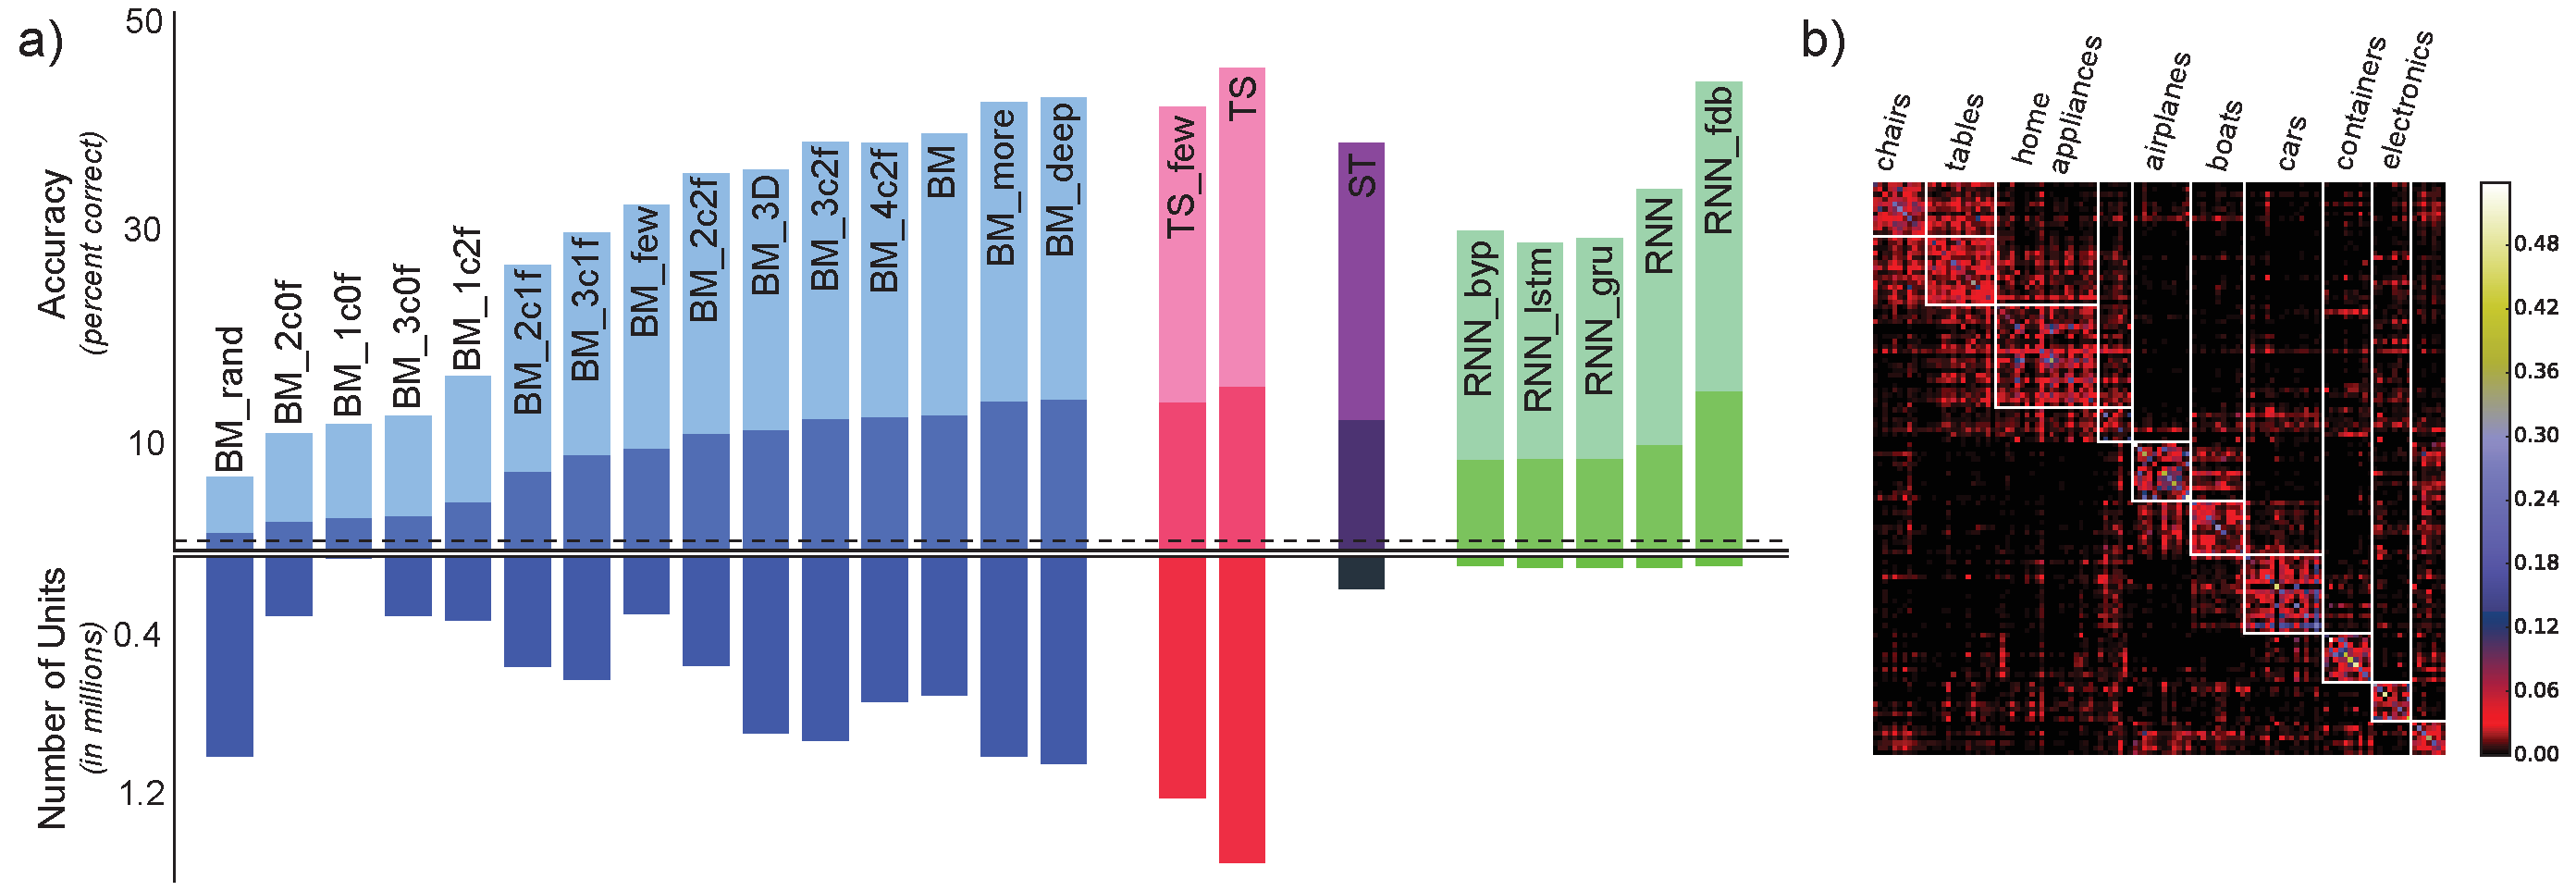
\includegraphics [width=1\linewidth]{figures/results.pdf}
\vspace{-3mm}
\caption{\footnotesize{\textbf{Performance results.} \textbf{a.} Each bar in this figure represents one model. The positive $y$-axis is performance measured in percent correct (top1=dark bar, chance=0.85\%, top5=light bar, chance=4.2\%).  The negative $y$-axis indicates the number of units in networks, in millions of units.  Small italic numbers indicate number of model parameters, in millions. Model architecture family is indicated by color. "ncmf" means n convolution and m fully connected layers. Detailed definition of individual model labels can be found in supplementary material. \textbf{b.} Confusion Matrix for the highest-performing model (in the Temporal-Spatial family). The objects are regrouped using methods described in supplementary material.}~\label{fig_main}}
\vspace{-5mm}
\end{figure}

\textbf{Model Performance:} 
Our strategy in identifying potential models of the whisker-trigeminal system is to explore many specific architectures within each architecture family, evaluating each specific architecture both in terms of its ability to solve the shape recognition task in our training dataset, and its efficiency (number of parameters and number of overall units).
Because it can be misleading to compare models with different numbers of parameters, we generally evaluated models with similar numbers of parameters: exceptions are noted where they occur.
As we evaluated many individual structures within each family, a list of the specific models and parameters are given in the supplementary materials.

Our results (Fig. \ref{fig_main}) can be summarized with following conclusions:

\begin{itemize}[leftmargin=*,itemsep=0ex,topsep=1ex]
   \item Many specific network choices within all families do a poor job at the task, achieving just-above-chance performance.
   \item However, within each family, certain specific choices of parameters lead to much better network performance.
   Overall, the best performance was obtained for the Temporal-Spatial model, with 15.2\% top-1 and 44.8\% top-5 accuracy.
   Visualizing a confusion matrix for this network (Fig. \ref{fig_main})b  and other high-performing networks indicate that the errors they make are generally reasonable.
   \item Training the filters was extremely important for performance; no architecture with random filters performed above chance levels.
   \item Architecture depth was an important factor in performance. Architectures with fewer than four layers achieved substantially lower performance than somewhat deeper ones.
   \item Number of model parameters was a somewhat important factor in performance within an architectural family, but only to a point, and not between architectural families.
   The Temporal-Spatial architecture was able to outperform other classes while using significantly fewer parameters.
   \item Recurrent networks with long-range feedback were able to perform nearly as well as the Temporal-Spatial model with equivalent numbers of parameters, while using far fewer units.
   These long-range feedbacks appeared critical to performance, with purely local recurrent architectures (including LSTM and GRU) achieving significantly worse results.
\end{itemize}

\textbf{Model Discrimination:}  The above results indicated that we had identified several high-performing networks in quite distinct architecture families.
In other words, the strong performance constraint allows us to identify several specific candidate model networks for the biological system, reducing a much larger set of mostly non-performing neural networks into a ``shortlist''.
The key biologically relevant follow-up question is then: how should we distinguish between the elements in the shortlist? 
That is, what signatures of the differences between these architectures could be extracted from data obtainable from experiments that use today's neurophysiological tools?

To address this question, we used Representational Dissimilarity Matrix (RDM) analysis~\cite{Kriegeskorte2008}.
For a set of stimuli $S$, RDMs are $|S| \times |S|$-shaped correlation distance matrices taken over the feature dimensions of a representation, e.g. matrices with $ij$-th entry $RDM[i, j] = 1 - corr(F[i], F[j])$ for stimuli $i, j$ and corresponding feature output $F[i], F[j]$.
The RDM characterizes the geometry of stimulus representation in a way that is independent of the individual feature dimensions.  RDMs can thus be quantitatively compared between different feature representations of the same data.
RDMs have been useful in establishing connections between deep neural networks and neural data from the ventral visual stream~\cite{cadieu2014deep, Yamins2014, khaligh2014deep}. 
RDMs are readily computable from neural response pattern data samples, and are in general are comparatively robust to variability due to experimental randomness (e.g. electrode/voxel sampling).
We obtained RDMs for several of our high-performing models, computing RDMs separately for each model layer (Fig. \ref{fig_rdms}a), averaging feature vectors over different sweeps of the same object before computing the correlations.
This procedure lead to $9981\times9981$-sized matrices (there were 9,981 distinct object in our dataset).
We then computed distances between each layer of each model in RDM space, as in (e.g.) \cite{khaligh2014deep}.
To determine if differences in this space between models and/or layers were significant, we computed RDMs for multiple instances of each model trained with different initial conditions, and compared the between-model to within-model distances.
We found that while the top layers of models partially converged (likely because they were all trained on the same task), intermediate layers diverged substantially between models, by amounts larger than either the initial-condition-induced variability within a model layer or the distance between nearby layers of the same model (Fig. \ref{fig_rdms}b).
This result is not entirely surprising since the models are quite structurally distinct.  
However, it establishes the initial computational validity for a conceptually simple and potentially feasible neuroscience experiment to distinguish between models: RDMs computed from neural recordings in multiple areas of the whisker-trigeminal system could be compared to model RDMs.

\begin{figure}
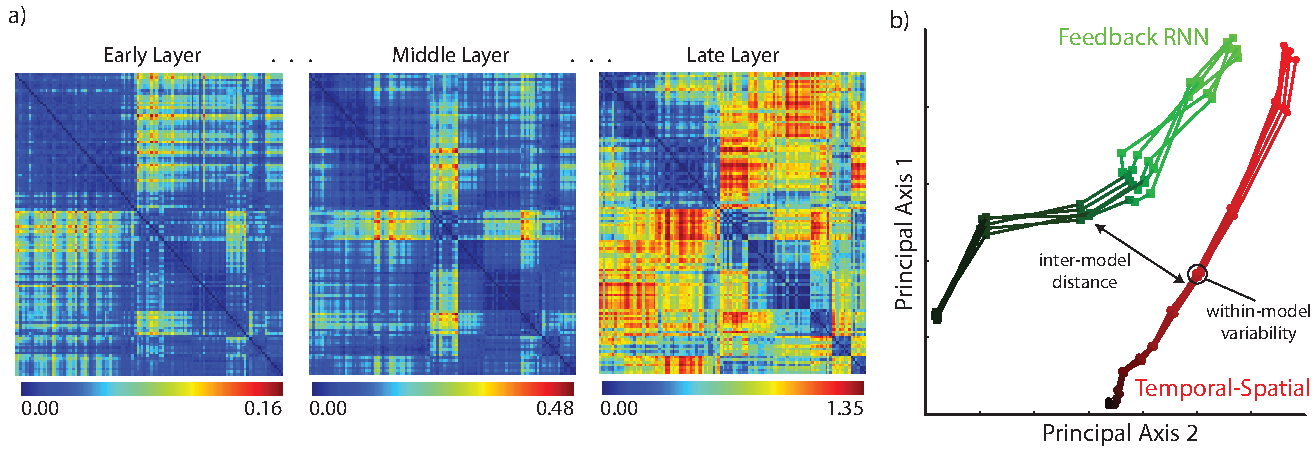
\includegraphics [width=1\linewidth]{figures/rdms.pdf}
\vspace{-5mm}
\caption{\footnotesize{\textbf{Using RDMs to Discriminate Between High-Performing Models.} \textbf{a.} Representational Dissimilarity Matrices (RDMs) for selected layers of a high-performing network from Fig. \ref{fig_main}a, showing early, intermediate and late model layers.  Model feature vectors are averaged over classes in the dataset prior to RDM computation, and RDMs are shown using the same ordering as in Fig. \ref{fig_main}b. \textbf{b.} Two-dimensional MDS embedding of RDMs for the feedback RNN (green squares) and Temporal-Spatial (red circles) model.  Points correspond to layers, lines are drawn between adjacent layers, with darker color indicating earlier layers.  Multiple lines are models trained from different initial conditions, allowing within-model noise estimate.}~\label{fig_rdms}}
\vspace{-5mm}
\end{figure}




\section{Conclusion}  %~250 words
We have introduced a model of the rodent whisker array informed by biophysical data, and used it to generate a large high-variability synthetic sweep dataset. 
While the raw sensor data is sufficiently powerful to separate objects at low amounts of variability, at higher variation levels deeper non-linear neural networks are required to extract object identity. 
We found further that while many particular network architectures, especially shallow ones, fail to solve the shape recognition task, reasonable performance levels can be obtained for specific architectures within each distinct network structural family tested.
We then showed that a population-level measurement that is in principle experimentally obtainable can distinguish between these higher-performing networks. 
To summarize, we have shown that a goal-driven DNN approach to modeling the whisker-trigeminal system is feasible. 
Code for all results, including the whisker model and neural networks, is publicly available at [WITHHELD].

We emphasize that the present work is proof-of-concept rather than a model of the real nervous system.
A number of critical issues must be overcome before our true goal --- a full integration of modeling with experimental data --- becomes possible.    
First, although our sensor model was biophysically informed, it does not include active whisking, and the mechanical signals at the whisker bases are approximate~\cite{Quist2014, Huet2016}.

An equally important problem is that the goal that we set for our network, i.e. shape discrimination between 117 human-recognizable object classes, is not directly ethologically relevant to rodents. 
The primary reason for this task choice was practical: ShapeNet is a readily available and high-variability source of 3D objects. 
If we had instead used a small, manually constructed, set of highly simplified objects that we hoped were more ``rat-relevant'', it is likely that our task would have been too simple to constrain neural networks at the scale of the real whisker-trigeminal system. 
Extrapolating from modeling of the visual system, training a deep net on 1000 image categories yields a feature basis that can readily distinguish between previously-unobserved categories~\cite{Yamins2014,cadieu2014deep,razavian2014cnn}.
Similarly, we suggest that the large and variable object set used here may provide a meaningful constraint on network structure, as the specific object geometries may be less important then having a wide spectrum of such geometries. 
However, a key next priority is systematically building an appropriately large and variable set of objects, textures or other class boundaries that more realistically model the tasks that a rodent faces.
The specific results obtained (e.g. which families are better than others, and the exact structure of learned representations) are likely to change significantly when these improvements are made.  

In the longer term, we expect to use detailed encoding models of the whisker-trigeminal system as a platform for investigating issues of representation learning and sensory-based decision making in the rodent. 
A particularly attractive option is to go beyond beyond fixed class discrimination problems and situate a synthetic whisker system on a mobile animal in a navigational environment where it will be faced with a variety of actively-controlled discrete and continuous estimation problems.
By doing this work with a rich sensory domain in rodents, we seek to leverage the sophisticated neuroscience tools available in these systems to go beyond what might would be possible in other model systems.  



%\begin{figure}[h]
%\centering
%\includegraphics [width=1\linewidth]{figures/model_class.pdf}
%\vspace{-2mm}
%\caption{\textbf{(a)} Figure caption~\label{figname}}
%\end{figure}


{\small
\bibliography{refs}}
\bibliographystyle{plain}

\end{document}
